% --------------------------------------------------------------
%                       Initialize
% --------------------------------------------------------------

\documentclass[11pt]{article}

\usepackage{personalNotes}
% contains special macros for math environment:
%     unit, p, set, abs, floor, ceil, vec, norm, inner, kernel
% contains useful all-purpose macros:
%     n, lessSeparation, append

\usepackage{tikz}
\usetikzlibrary{shapes,snakes}
\newcommand{\tedge}[5]{\draw[#3] (#1)-- node[e, #5] (e#4) {#4} (#2)}

% --------------------------------------------------------------
%                    Beginning of Document
% --------------------------------------------------------------

\begin{document}

% --------------------------------------------------------------
%                           Title
% --------------------------------------------------------------

\pntitle {Graph Theory}
\pnauthor{Troy Baker}
\pndate  {May 13, 2014}


\pnmaketitle
\pnmakefooter

% --------------------------------------------------------------
%                           Body
% --------------------------------------------------------------

\section{Definitions}
\begin{definition}[Graph]
Graph $G=(V,E)$ is a set of vertices, $V$, and a set of edges, $E$, defined as a tuple of vertices from $V$. Additionally, there are two weight functions, $w_V: V \to \mathbb{R}$ and $w_E: E \to \mathbb{R}$.
\end{definition}

\begin{definition}[Density]
The density of a graph is defined as:
\[d(G) = \sum_{v\in V}{w_V(v)} - \sum_{e\in E}{w_E(e)}\]
\end{definition}

\begin{definition}[Underconstrained Graph]
Graph $G=(V,E)$ is underconstrained if, given constant $k$, $d(G) > k$.
\end{definition}

\begin{definition}[Overconstrained Graph]
Graph $G=(V,E)$ is overconstrained if, given constant $k$, $d(G) < k$.
\end{definition}

\begin{definition}[Wellconstrained Graph]
Graph $G=(V,E)$ is wellconstrained if, given constant $k$ and a set of trivial graphs $T$, the graph satisfies (1) $d(G)=k$ and (2) all subgraphs are either underconstrained, wellconstrained, or trivial (i.e.\ are isomorphic to one of the graphs in $T$).
\end{definition}

\begin{definition}[Trivial Graph]
A trivial graph is ill-defined in the general case. The only strict requirements are: (1) it must be an overconstrained graph and (2) all of its subgraphs are also trivial.

In the familiar geometric cases of $d$-dimensional space, all vertex weights are $d$, all edge weights are $1$, and constant $k= {{d+1}\choose{2}}$. Trivial graphs for 2D would be a single vertex. Trivial graphs in 3D would be a vertex and an edge (2 vertices with an edge between). Etc. These trivial graphs capture the notion of the rotational symmetry that exists in geometric spaces.
\end{definition}

\begin{definition}[Decomposition Recombination (DR-) Plan]
A DR-plan of graph $G$, $DRP(G)$, is a tree that has the following properties:
\begin{enumerate}
    \item The root of the tree `contains' $G$.
    \item For all nodes, $C$, that `contain' nontrivial graphs, its $N$ children, $C_1, \ldots, C_N$, are either trivial subgraphs or wellconstrained vertex-maximal proper subgraphs of that node $C$.
    \item $\bigcup_{i=1}^N{C_i}=C$.
    \item OR IS IT..... The vertex set of $\bigcup_{i=1}^N{C_i}$ has all the vertices that are in $C$.
\end{enumerate}

% It can also be described recursively as: the root is $G$, its children are the trivial subgraphs and the DR-plans of its wellconstrained vertex-maximal proper subgraphs whose union is $G$ itself.

An equivalent DAG can be constructed from this tree such that all nodes containing the same subgraphs are combined into one, with all edges preserved.

Note that nodes will be referred to interchangeably as ``the node that contains the (sub)graph $C$'' and as simply ``$C$''.
\end{definition}


\begin{definition}[Optimal DR-Plan]
The optimal DR-plan of graph $G$, $OPTDRP(G)$, is the DR-plan that minimizes the maximum fan-in over all nodes in the tree/DAG.
\end{definition}




\section{Notation}
$G$ is taken to be a graph with vertex set $V$ and edge set $E$.

$Idc(G,X)$ is the graph induced on $G$ with the vertex set $X\subseteq V$. This can also be overloaded such that, using graph $H=(W,F)$, $Idc(G,H)=Idc(G,W)$.

$C$ is an arbitrary graph in a node in $DRP(G)$. $C_i$ is the $i^{\text{th}}$ child of $C$ (implied to be a wellconstrained vertex-maximal proper subgraph, by definition of a DR-plan).




\section{The Canonical Optimal DR-Plan}
\begin{figure}
\begin{center}
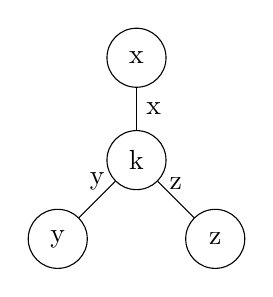
\begin{tikzpicture}
    \tikzstyle{v}=[draw, circle, minimum size=0.75cm]
    \tikzstyle{e}=[]

    \node[v] (v1) at (1,1) {y};
    \node[v] (v2) at (3,1) {z};
    \node[v] (v3) at (2,2) {k};
    \node[v] (v4) at (2,3.3) {x};

    \tedge{v1}{v3}{solid}{y}{above};
    \tedge{v2}{v3}{solid}{z}{above};
    \tedge{v3}{v4}{solid}{x}{right};

    % \draw (3.3,2.5) circle (1.9cm);
    % \draw (.7,2.5) circle (1.9cm);
    % \draw (2,.5) circle (1.9cm);
\end{tikzpicture}
\\
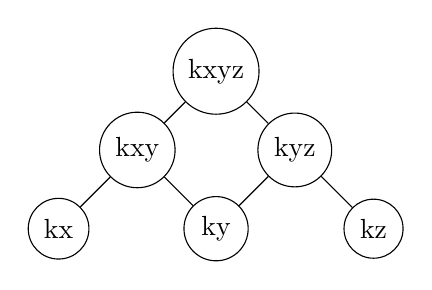
\begin{tikzpicture}
    \tikzstyle{v}=[draw, circle, minimum size=0.75cm]
    \tikzstyle{e}=[]

    \node[v] (v1) at (0,  0) {kxyz};
    \node[v] (v2) at (-1,-1) {kxy};
    \node[v] (v3) at ( 1,-1) {kyz};
    \node[v] (v4) at (-2,-2) {kx};
    \node[v] (v5) at ( 0,-2) {ky};
    \node[v] (v6) at ( 2,-2) {kz};

    \tedge{v1}{v2}{solid}{}{};
    \tedge{v1}{v3}{solid}{}{};
    \tedge{v2}{v4}{solid}{}{};
    \tedge{v2}{v5}{solid}{}{};
    \tedge{v3}{v5}{solid}{}{};
    \tedge{v3}{v6}{solid}{}{};
\end{tikzpicture}
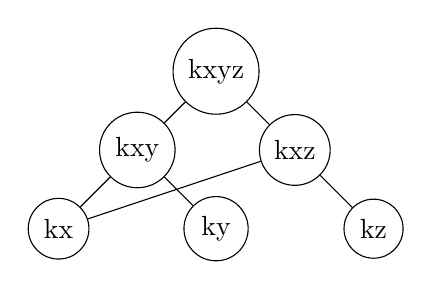
\begin{tikzpicture}
    \tikzstyle{v}=[draw, circle, minimum size=0.75cm]
    \tikzstyle{e}=[]

    \node[v] (v1) at (0,  0) {kxyz};
    \node[v] (v2) at (-1,-1) {kxy};
    \node[v] (v3) at ( 1,-1) {kxz};
    \node[v] (v4) at (-2,-2) {kx};
    \node[v] (v5) at ( 0,-2) {ky};
    \node[v] (v6) at ( 2,-2) {kz};

    \tedge{v1}{v2}{solid}{}{};
    \tedge{v1}{v3}{solid}{}{};
    \tedge{v2}{v4}{solid}{}{};
    \tedge{v2}{v5}{solid}{}{};
    \tedge{v3}{v4}{solid}{}{};
    \tedge{v3}{v6}{solid}{}{};
\end{tikzpicture}
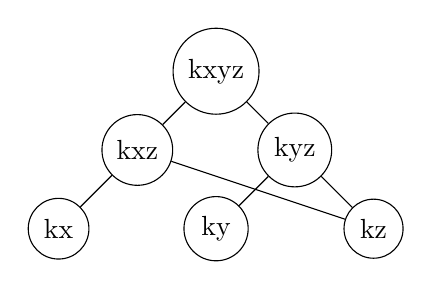
\begin{tikzpicture}
    \tikzstyle{v}=[draw, circle, minimum size=0.75cm]
    \tikzstyle{e}=[]

    \node[v] (v1) at (0,  0) {kxyz};
    \node[v] (v2) at (-1,-1) {kxz};
    \node[v] (v3) at ( 1,-1) {kyz};
    \node[v] (v4) at (-2,-2) {kx};
    \node[v] (v5) at ( 0,-2) {ky};
    \node[v] (v6) at ( 2,-2) {kz};

    \tedge{v1}{v2}{solid}{}{};
    \tedge{v1}{v3}{solid}{}{};
    \tedge{v2}{v4}{solid}{}{};
    \tedge{v2}{v6}{solid}{}{};
    \tedge{v3}{v5}{solid}{}{};
    \tedge{v3}{v6}{solid}{}{};
\end{tikzpicture}
% \\
% \begin{tikzpicture}
%     \tikzstyle{v}=[draw, circle, minimum size=0.75cm]
%     \tikzstyle{e}=[]

%     \node[v] (v1) at ( 0, 0) {kxyz};
%     \node[v] (v2) at (-1,-1) {kxy};
%     \node[v] (v3) at (-2,-2) {kx};
%     \node[v] (v4) at (-3,-3) {k};
%     \node[v] (v5) at ( 1,-1) {z plan};
%     \node[v] (v6) at ( 0,-2) {y plan};
%     \node[v] (v7) at (-1,-3) {x plan};
%     \node[v] (v8) at (-2,-4) {k plan};

%     \tedge{v1}{v2}{solid}{}{};
%     \tedge{v1}{v5}{solid}{}{};
%     \tedge{v2}{v3}{solid}{}{};
%     \tedge{v2}{v6}{solid}{}{};
%     \tedge{v3}{v4}{solid}{}{};
%     \tedge{v3}{v7}{solid}{}{};
%     \tedge{v4}{v8}{solid}{}{};
% \end{tikzpicture}
\end{center}

\caption{A wellconstrained graph whose nodes are subgraphs labeled with their density. Below are its 3 optimal DR-Plans (partially complete). The center vertex has weight $k$ and is wellconstrained itself. The radial nodes have weights $x,y,z \neq k$ with equivalent edge weights, making any union between $k$ and the others wellconstrained.}
\label{3-plans}
\end{figure}

In the case of a wellconstrained graph, it is clear that there always exists a single vertex-maximum DR-Plan that includes every single wellconstrained vertex-maximal proper subgraph at each node. However, in the problem of the optimal DR-Plan there is no such unique plan. For instance, a graph that is formed by the union of 3 wellconstrained subgraphs that all intersect on a wellconstrained subgraph, demonstrated in Figure \ref{3-plans}. In this case, it results in $3$ unique optimal DR-Plans. Indeed, we will prove a union of $N$ wellconstrained subgraphs will result in $N$ unique plans, but that at the $N^{\text{th}}$ level of the tree it will always be the same. Therefore, all choices of decomposition are in some sense equivalent.

We develop this notion of the canonical optimal DR-plan by carefully considering the case of a union of any two nontrivial wellconstrained vertex-maximal proper subgraphs of a wellconstrained graph. By definition, any subgraph of a wellconstrained graph will either be (1) trivial, (2) underconstrained, or (3) wellconstrained. We will analyze all 3 possibilities in turn.

% We show this by carefully considering all of the potential cases of the unions of subgraphs. By definition, any subgraph of a wellconstrained graph will either be (1) underconstrained, (2) wellconstrained, or (3) trivial. We will analyze all 3 possibilities in turn, in the case of a union of any two nontrivial wellconstrained vertex-maximal proper subgraphs.


\subsection{Union is Trivial}
\begin{lemma}
The union of wellconstrained graphs cannot result in a trivial graph.
\end{lemma}

\begin{proof}
% If $C_i,C_j$ are wellconstrained, then $C_i\cup C_j \geq k$. Trivial graphs must be overconstrained.

Follows from the definition of a trivial graph. It would imply that the wellconstrained graphs were also trivial.
\end{proof}


\subsection{Union is Underconstrained}
\begin{lemma}\label{uc-l1}
Given two wellconstrained subgraphs $C_i,C_j$, $C_i\cup C_j$ is underconstrained if and only if $C_i\cap C_j$ is trivial.
\end{lemma}

\begin{proof}
This can be shown with simple arithmetic. It follows from definitions that $d(C_i)=k$ and $d(C_j)=k$. In the forward direction we have that $d(C_i\cup C_j)=l>k$, therefore $d(C_i\cap C_j)=d(C_i)+d(C_j)-d(C_i\cup C_j)=2k-l<k$. The only way to have an overconstrained subgraph in a wellconstrained graph is if it is trivial. In the backwards direction the same math proves it.
\end{proof}

\begin{lemma}
If there exist $C_i, C_j$ such that $C_i\cap C_j$ is trivial, then for all $C_k,C_l$, $C_k\cap C_l$ is trivial or empty set.
\end{lemma}

\begin{proof}
Suppose
\end{proof}

\begin{figure}
\begin{center}
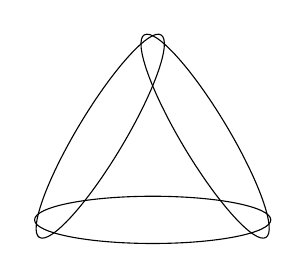
\begin{tikzpicture}
    \draw[rotate=0]  (0,0) ellipse (1.5cm and .3cm);
    \draw[rotate around={-59:(.7,1.2)}] (.8,1.1) ellipse (1.5cm and .3cm);
    \draw[rotate around={59:(-.7,1.2)}] (-.8,1.1) ellipse (1.5cm and .3cm);

    % \draw[rotate around={59:(.7,-1.2)}] (.8,-1.1) ellipse (1.5cm and .3cm);
    % \draw[rotate around={-59:(-.7,-1.2)}] (-.8,-1.1) ellipse (1.5cm and .3cm);

    % \draw[rotate=0] (1,1) ellipse (.1cm and .1cm);
    % \draw[rotate=66] (0,0) ellipse (.1cm and .1cm);
\end{tikzpicture}
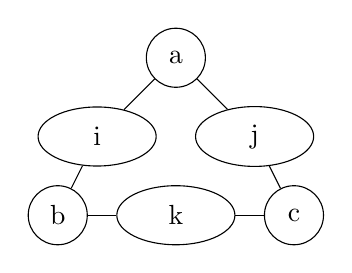
\begin{tikzpicture}
    \tikzstyle{v}=[draw, circle, minimum size=0.75cm]
    \tikzstyle{el}=[draw, ellipse, minimum height=.75cm, minimum width=1.5cm]
    \tikzstyle{e}=[]

    \node[el] (m) at (0,    0) {k};
    \node[v]  (l) at (-1.5, 0) {b};
    \node[v]  (r) at (1.5,  0) {c};

    \node[el] (tl) at (-1,  1) {i};
    \node[el] (tr) at (1,   1) {j};
    \node[v]  (t)  at (0,   2) {a};

    % \node[el] (bl) at (-1,  -1) {l};
    % \node[el] (br) at (1,   -1) {m};
    % \node[v]  (b)  at (0,   -2) {d};

    % \node[el] (v2) at (-1,-1) {b};
    % \node[el] (v3) at (-1,-1) {b};
    % \node[el] (v4) at (-1,-1) {b};
    % \node[el] (v5) at (-1,-1) {b};

    \tedge{m}{l}{solid}{}{};
    \tedge{m}{r}{solid}{}{};

    \tedge{l}{tl}{solid}{}{};
    \tedge{tl}{t}{solid}{}{};
    \tedge{r}{tr}{solid}{}{};
    \tedge{tr}{t}{solid}{}{};

    % \tedge{l}{bl}{solid}{}{};
    % \tedge{bl}{b}{solid}{}{};
    % \tedge{r}{br}{solid}{}{};
    % \tedge{br}{b}{solid}{}{};
\end{tikzpicture}
\end{center}

\caption{Each node contains a subgraph of the entire, wellconstrained graph. We take $a\cup i\cup b$, $a\cup j\cup c$, and $b\cup k\cup c$ to be wellconstrained. If the union of any two of these listed unions is underconstrained then it immediately follows that all such unions are underconstrained and that nodes $a,b,c$ must all be trivial subgraphs.
THIS IS NOT TECHNICALLY CORRECT... $a\cup i\cup b$ doesn't include the edge between them... Is there a better way to phrase this?
% Each node contains a subgraph of the entire, wellconstrained graph. We take $a\cup i\cup b$, $a\cup j\cup c$, $b\cup k\cup c$, $b\cup l\cup d$, and $c\cup m\cup d$ to be wellconstrained. If the union of any two of these listed unions is underconstrained then it immediately follows that all such unions are underconstrained and that nodes $a,b,c,d$ must all be trivial subgraphs.
% THIS IS NOT TECHNICALLY CORRECT... $a\cup i\cup b$ doesn't include the edge between them... Is there a better way to phrase this?
}
\label{trivial-intersection}
\end{figure}


\begin{theorem}\label{uc-t1}
% In any solution to $OPTDRP(G)$, if any two wellconstrained vertex-maximal proper subgraphs of a node form a union that is underconstrained, then all wellconstrained vertex-maximal proper subgraphs of said node must be included in the optimal plan.

In $OPTDRP(G)$ of a wellconstrained $G$, if $C_i \cap C_j$ is trivial, then all $C_1,\ldots, C_N$ must be included in the optimal plan as children of $C$.
\end{theorem}

\begin{proof}
From Lemma \ref{uc-l1}, if it is trivial then $C_i \cup C_j$ must be underconstrained. If it is underconstrained, it must be part of some larger wellconstrained subgraph $D$. If $D$ is not $G$ itself, then we just found a larger proper subgraph and the graphs in the set were not vertex-maximal to begin with.
 For $C$ to be wellconstrained... WHAT????

If there was some $X\subset [1,\ldots,N]$ such that $\bigcup_{i\in X}{C_i}\neq C$ but it was wellconstrained, then we just found a larger proper subgraph and the graphs in the set were not vertex-maximal to begin with.

This means that in the case of a trivial intersection, all of the children come together to form some complex structure that is itself rigid. Such an example is shown in Figure \ref{trivial-intersection}.
\end{proof}

% As such, there must be additional vertex-maximal proper subgraphs, all of whose intersections with one another are trivial subgraphs or $\emptyset$. All of these subgraphs form a complex structure that is wellconstrained and must be the parent itself (otherwise we did not have vertex-maximal subgraphs to begin with).







\subsection{Union is Wellconstrained}

\begin{lemma}
Given two wellconstrained subgraphs $C_i,C_j$, $C_i\cup C_j$ is wellconstrained if and only if $C_i\cap C_j$ is wellconstrained.
\end{lemma}

\begin{proof}
In the forward direction: From Lemma \ref{uc-l1}, the intersection cannot be trivial. The intersection also cannot be underconstrained. If $C_i \cap C_j$ were underconstrained, then for $C_i$ to be wellconstrained you would need to add more constraints (edge weight) than degrees of freedom (vertex weight) to the intersection. The same is true for $C_j$. If both of these were satisfied, then the union of $C_i$ and $C_j$ would result in an overconstrained nontrivial graph. This is a contradiction, by definition of a wellconstrained graph. Therefore, the intersection can only be wellconstrained.

BACKWARDS!!!!!
\end{proof}

\begin{lemma}\label{wc-l2}
Given two wellconstrained vertex-maximal proper subgraphs $C_i, C_j$, $C_i\cup C_j$ is wellconstrained if and only if $C_i\cup C_j = C$.
\end{lemma}

\begin{proof}
The forwards direction can be shown with a contradiction. If the $C_i\cup C_j$ was wellconstrained but $C_i\cup C_j \neq C$, we would have found a larger wellconstrained proper subgraph containing them; namely, $C_i\cup C_j$ or something containing it would have been larger. The two original subgraphs could not have been vertex-maximal proper.

The backwards direction follows from the definition of a DR-plan.
\end{proof}

\begin{theorem}\label{wc-t1}
% In $OPTDRP(G)$ of a wellconstrained $G$, if any two wellconstrained vertex-maximal proper subgraphs of a node form a union that is wellconstrained, then said node can have only $2$ children.

In $OPTDRP(G)$ of a wellconstrained $G$, if $C_i \cup C_j$ is wellconstrained, then any 2 wellconstrained vertex-maximal proper subgraphs of $C$ will be sufficient as its children.
% Namely, these children are any 2 of its wellconstrained vertex-maximal proper subgraphs.
\end{theorem}

\begin{proof}
For a valid DR-plan, all children must be proper subgraphs. Therefore, for the union to be the parent (and satisfy the conditions of a DR-plan) there must be at least 2 children. It follows directly from Lemma \ref{wc-l2} that if there exists $C_i, C_j$ such that $C_i \cup C_j$ is wellconstrained, then you found a tree with only 2 children.

Clearly, this is the optimal choice at this level. However, for it to be a solution to $OPTDRP(G)$, it must not affect the maximum fan-in later on.

Take $\bigcap_{k=1}^N{C_k}$ to be the graph $D$. Take $C\setminus C_k$ to be $F_k$.

After we go down $N$ levels we get to a point where every node is some $F_k$ with $D$ and all the edges connecting them.

This is demonstrated with $N=3$ in Figure \ref{3-plans}. It is clear that until this point, the fan-in at every node is exactly 2 in the optimal solution. This follows from the discussion above. Now, at this level, the fan-in must be equal in all scenarios. In fact, at node $k$ it will be 1 (because of $D$ which is wellconstrained) plus whatever fan-in $F_k$ incurs.
\end{proof}


% (2) If the union results in a wellconstrained subgraph, it must be the entire graph. If this were not the case, .

% More can be said about the intersection of these two subgraphs, $C_1=(V_1, E_1)$ and $C_2=(V_2, E_2)$. It cannot be overconstrained, otherwise the union could not be wellconstrained (simple arithmetic, see the first case).

\begin{corollary}
Take $\bigcap_{k=1}^N{C_k}$ to be the graph $D$. If $D$ is wellconstrained, then $D$ will be a descendant of every $C_k$.
\end{corollary}

\begin{proof}
Explained in Theorem \ref{wc-t1}.
\end{proof}

\begin{corollary}
$\forall i,j\in [1,\ldots,N]$ if $i\neq j$ there are no edges in $C$ between the vertices in subgraphs $C\setminus C_i$ and $C\setminus C_j$.
\end{corollary}

\begin{proof}
Further constraints between them would imply $C_i \cup C_j$ is a subgraph of $C$, but lemma \ref{wc-l2} proves is the entire graph.
\end{proof}

% \begin{proof}
% It follows from Theorem \ref{uc-t1} that if the intersection of any two wellconstrained vertex-maximal proper subgraphs of $C$ are wellconstrained then all of them are wellconstrained or $\emptyset$.
% \end{proof}

% Figure idea: Large node in the middle with weight $k$. Several other graphs with weight $a, b, c, d\ldots$ attached radially by single edges with weights $a, b, c, d\ldots$ respectively. Circle each vertex-maximal subset.

% $\forall k\in [1,\ldots,N]$ the subgraphs $C\setminus C_k$ will be edge disjoint. Therefore the solving of one is exclusive of the solving of the other.

% Furthermore, the union of all of these subgraphs will be $C\setminus D$. So each subgraph will need to be ``tacked'' onto $D$ for recombination and since they are edge-disjoint the order is unimportant.





% \pnplaceholder
% \begin{lemma}
% If $C_1$ and $C_2$ are wellconstrained vertex-maximal proper subgraphs of $C$ and $C_1 \cap C_2$ is wellconstrained, then $C_1 \cap C_2$ is a wellconstrained vertex-maximal proper subgraph of every child of $C$.
% \end{lemma}

% \begin{proof}
% First, it must be a vertex-maximal proper subgraph of $C_1$ and $C_2$. Say that there was some larger proper subgraph in $C_1$ that was well constrained. If this were true, then $C_2$ was not vertex-maximal because it could have included that entire subgraph and remained wellconstrained. The same is true vice versa.

% Second, the discussion in the proof of the theorem holds true for any two subgraphs. Therefore, the same intersection is present in all of them.
% \end{proof}
% \pnplaceholder





\subsection{Further Results}

% \begin{corollary}
% There are no edges between $V_1 \setminus (V_1\cap V_2)$ and $V_2 \setminus (V_1\cap V_2)$.
% \end{corollary}

% \begin{proof}
% As a result of the discussion of the second part, it is clear that there cannot be any further constraints between $V_1 \setminus (V_1\cap V_2)$ and $V_2 \setminus (V_1\cap V_2)$. That would imply $C_1 \cup C_2$ is a subgraph, but we know it to be the entire graph.
% \end{proof}



\begin{corollary}
There is no rigid subgraph induced by a proper, nonempty subset of vertices of $V_i \setminus (V_1\cap V_2)$ and a subset of $V_1\cap V_2$ of size at least 2.
\end{corollary}

\begin{proof}
Since $C_1\cup C_2$ is the entire graph, PROVE THIS!!!!
\end{proof}




% \begin{corollary}
% If $C_1$ and $C_2$ are wellconstrained vertex-maximal proper subgraphs of $C$ and $C_1 \cap C_2$ is wellconstrained, then $C_1 \cap C_2$ is a wellconstrained vertex-maximal proper subgraph of every child of $C$.
% \end{corollary}

% \begin{proof}
% First, it must be a vertex-maximal proper subgraph of $C_1$ and $C_2$. Say that there was some larger proper subgraph in $C_1$ that was well constrained. If this were true, then $C_2$ was not vertex-maximal because it could have included that entire subgraph and remained wellconstrained. The same is true vice versa.

% Second, the discussion in the proof of the theorem holds true for any two subgraphs. Therefore, the same intersection is present in all of them.
% \end{proof}



\section{Future Work}
While this paper fleshes out the case of a wellconstrained input graph, little work has been done on the overconstrained graph. This has to do with the fact that finding a DR-Plan is NP-complete.

Underconstrained is not worth studying in itself, because it will either be that all subgraphs are underconstrained or trivial or that some subgraphs are wellconstrained or overconstrained. In this sense, it is not an independent problem.










% \section{Formal Conjectures}

% \subsection{Conjecture 1}



% \begin{conjecture}
% % Take $G$ to be wellconstrained. Then, for all nodes $C$ in $DRP(G)$, either $\forall i,j (C_i \cap C_j \leq 1)$ or $\forall i,j (C_i \cap C_j \geq 2) \wedge (C_i \cup C_j = C)$.

% % or...

% Take $G$ to be wellconstrained. The operator $\cap_V$ returns the count of the vertices in the intersection of two graphs. Then, for all nodes $C$ in $DRP(G)$, exactly one of the following is true:
% \begin{align*}
%     \forall i,j & (C_i \cap_V C_j = 1) \wedge \p{\bigcup_{k\in\set{1,\ldots,N}\setminus\set{i}}{C_k} \neq C} \text{ or} \\
%     \forall i,j & (C_i \cap_V C_j \geq 2) \wedge (C_i \cup C_j = C)
% \end{align*}


% That is, either any two children share a single vertex and all of them are needed to form the parent node, or there is some significant overlap of 2 or more vertices and because of that only 2 children are needed at node $C$ to satisfy the definition of the DR-plan.

% This implies that in the first scenario all proper vertex-maximal rigid subgraphs of $C$ must be in tree $DRP(C)$, and that in the second scenario only 2 such subgraphs need to be in the tree.

% $C_i \cap_V C_j$ cannot be $<1$ because 0 is disjoint but $G$ is taken to be wellconstrained (negative and non-integral values are meaningless).
% \end{conjecture}

% \begin{conjecture}
% $DRP(G)$ is ``unique'' modulo choice of children. Which means that the choice of children cannot impact the solution of the framework.
% \end{conjecture}



\pnplaceholder
Notes:
Edges do not appear as nodes of the DR plan, although vertices do (as leaves). In general, the children of a node are well-constrained proper maximal subgraphs of the parent, whose vertex set union gives the parent's vertex set.

We are trying to formalize here the concept of a canonical DR-plan of a well-constained graph; i.e, whether the non-uniqueness of the decomposition - in the case that some pair of proper vertex maximal rigid subgraphs have a nontrivial intersection - makes any real difference.

Conjecture 1 (should be easy to prove):
Let $C = (V,E)$ be well-constrained and $C_1 =(V_1,E_1),C_2 = (V_2,E_2)$ any two proper vertex-maximal well-constrained subgraphs with $V = V_1\cup V_2$ and $|V_1\cap V_2| \ge 2$ (called a nontrivial intersection). Then the subgraph $S_{1,2}$ induced by $V_1\cap V_2$ must be wellconstrained.


Here are corollary facts that should be easy to prove:
(1) There are no edges between $V_1 \setminus (V_1\cap V_2)$ and $V_2 \setminus (V_1\cap V_2)$.
(2) There is no rigid subgraph induced by a proper, nonempty subset of vertices of   $V_i \setminus (V_1\cap V_2)$ and a subset of $V_1\cap V_2$ of size at least 2.

Corollary of Conjecture 1 and resulting facts:
$C_1\cap C_2$ is a proper vertex maximal rigid subgraph of $C_i$. Either there is a unique second proper vertex maximal rigid subgraph of $C_i$ that intersects  $C_1\cap C_2$  nontrivially (on an edge), or every pair of proper vertex maximal rigid subgraphs of $C_i$ intersect trivially.

This would imply the DR-plans of $C_1$ and $C_2$ will be unique and have a common child in the DR-plan of $C_1\cap C_2$.

Conjecture 2: Let $C = (V,E)$ be well-constrained and $C_1 =(V_1,E_1),C_2 = (V_2,E_2)$ any two proper vertex-maximal well-constrained subgraphs with $V = V_1\cup V_2$ and $|V_1\cap V_1| \ge 2$. $C_3 =(V_3,E_3),C_4 = (V_4,E_4)$ any two proper vertex-maximal well-constrained subgraphs with $V = V_3\cup V_4$ and $|V_3\cap V_4| \ge 2$. Then both DR-plans where $C_1$ and $C_2$ are taken as children or where $C_4$ and $C_3$ are taken as children will have the same max fan-in. In particular, either DR-plan will contain $\bigcap\limits_i C_i$ as a node - at the 2nd level below $C$.

% \pnplaceholder

% Lemma 1: if the graph is wellconstrained and any two proper vertex maximal subgraphs have an overlap of only one vertex, then all of the subgraphs will have 1 or 0.

% Overlap of one vertex between any $C_i$ and $C_j$ means that $C\neq C_i\cup C_j$ because we know $C$ is wellconstrained and the graph $C_i\cup C_j$ would be able to pivot around the single vertex.

% \pnplaceholder

% Need to define trivial as a graph that, were it only accounting for vertices, would be overconstrained. I.e.\ a single vertex in 2D. Or a vertex and an edge in 3D.

% \pnplaceholder

% \begin{theorem}
% phrasing...
% \end{theorem}

% \begin{proof}
% By definition, any subgraph of a wellconstrained graph will either be (1) underconstrained, (2) wellconstrained itself, or (3) an overconstrained graph, referred to as trivial. We will analyze all 3 possibilities in turn, in the case of a union of any two nontrivial wellconstrained vertex-maximal proper subgraphs.

% (1) If the union results in an underconstrained subgraph, then the intersection of the two original subgraphs must be an overconstrained trivial subgraph (can be shown with simple arithmetic). As such, there must be additional vertex-maximal proper subgraphs, all of whose intersections with one another are overconstrained trivial subgraphs (including $\emptyset$). All of these edge-disjoint subgraphs form a complex structure that is wellconstrained and must be the graph itself (otherwise we did not have vertex-maximal subgraphs to begin with).

% (2) If the union results in a wellconstrained subgraph, it must be the entire graph. If this were not the case, the two original subgraphs could not have been vertex-maximal proper because we would have found a larger wellconstrained subgraph containing them; namely, their union or something containing it would have been larger.

% More can be said about the intersection of these two subgraphs, $C_1=(V_1, E_1)$ and $C_2=(V_2, E_2)$. It cannot be overconstrained, otherwise the union could not be wellconstrained (simple arithmetic, see the first case). The intersection also cannot be underconstrained. If $C_1 \cap C_2$ were underconstrained, then for $C_1$ to be wellconstrained you would need to add more constraints (edge weight) than degrees of freedom (vertex weight) to the intersection. The same is true for $C_2$. If both of these were satisfied, then the union of $C_1$ and $C_2$ would result in an overconstrained nontrivial graph. This is a contradiction, because we have shown the union to be the graph itself, which was defined to be wellconstrained. Therefore, the intersection must be wellconstrained.

% (3) It is impossible for the union of 2 nontrivial subgraphs to be trivial.
% \end{proof}




% \begin{corollary}
% There are no edges between $V_1 \setminus (V_1\cap V_2)$ and $V_2 \setminus (V_1\cap V_2)$.
% \end{corollary}

% \begin{proof}
% As a result of the discussion of the second part, it is clear that there cannot be any further constraints between $V_1 \setminus (V_1\cap V_2)$ and $V_2 \setminus (V_1\cap V_2)$. That would imply $C_1 \cup C_2$ is a subgraph, but we know it to be the entire graph.
% \end{proof}



% \begin{corollary}
% There is no rigid subgraph induced by a proper, nonempty subset of vertices of $V_i \setminus (V_1\cap V_2)$ and a subset of $V_1\cap V_2$ of size at least 2.
% \end{corollary}

% \begin{proof}
% Since $C_1\cup C_2$ is the entire graph,

% well... no. if $V_i$ contains $V_1 \setminus (V_1\cap V_2)$ or $V_2 \setminus (V_1\cap V_2)$, then you will induce a wellconstrained graph.
% \end{proof}




% \begin{corollary}
% $C_1 \cap C_2$ is a wellconstrained vertex-maximal proper subgraph of every $C_i$.
% \end{corollary}

% \begin{proof}
% First, it must vertex-maximal proper subgraph of $C_1$ and $C_2$. Say that there was some larger proper subgraph in $C_1$ that was well constrained. If this were true, then $C_2$ was not vertex-maximal because it could have included that entire subgraph and remained wellconstrained. The same is true vice versa.

% Second, the discussion in the proof of the theorem holds true for any two subgraphs. Therefore, the same intersection is present in all of them.
% \end{proof}

% \pnplaceholder



% \pnplaceholder

% need to show that that intersection is going to end up being a vertex-maximal subgraph of both of the original subgraphs. As a result, in the second case it doesn't matter which 2 you took.



% --------------------------------------------------------------
%                        End of Body
% --------------------------------------------------------------

\end{document}

% --------------------------------------------------------------
%                       End of Document
% --------------------------------------------------------------
